% Created 2025-04-29 Tue 19:24
% Intended LaTeX compiler: pdflatex
\documentclass[11pt]{article}
\usepackage[utf8]{inputenc}
\usepackage[T1]{fontenc}
\usepackage{graphicx}
\usepackage{longtable}
\usepackage{wrapfig}
\usepackage{rotating}
\usepackage[normalem]{ulem}
\usepackage{amsmath}
\usepackage{amssymb}
\usepackage{capt-of}
\usepackage{hyperref}
\usepackage{minted}
\usepackage{graphicx, array, siunitx, forest}
\graphicspath{ {./images/} }
\author{Hankertrix}
\date{\today}
\title{Entry To Biology Notes}
\hypersetup{
 pdfauthor={Hankertrix},
 pdftitle={Entry To Biology Notes},
 pdfkeywords={},
 pdfsubject={},
 pdfcreator={Emacs 30.1 (Org mode 9.7.11)}, 
 pdflang={English}}
\begin{document}

\maketitle
\setcounter{tocdepth}{2}
\tableofcontents \clearpage\newpage
\section{Definitions}
\label{sec:org90b393e}

\subsection{Trace elements}
\label{sec:org348e56c}
Trace elements are just elements that are found in small amounts in biological systems. They are usually not important to biological processes.
\subsection{Electronegativity}
\label{sec:org3667862}
Electronegativity describes the relative ability of an atom to attract electrons in a covalent bond. It is a dimensionless quantity, which means it is not quantifiable.
\subsection{Polarity}
\label{sec:orgefc1537}
Polarity refers the difference in electronegativity between two atoms in a covalent bond.


A polar bond is one that has two atoms of different electronegativities, which will result in the more electronegative atom pulling the electrons towards its nucleus, increasing the electron density around itself and making the bond polar.


A non-polar bond is one that has two atoms of similar electronegativity, which results in the atoms exerting a similar pull on the electrons, making the bond non-polar.
\subsection{Ionic bond}
\label{sec:org9e7b166}
Oppositely charged ions formed through the loss or gain of electrons are strongly attracted to each other, forming ionic bonds. Compounds with ionic bonds usually form a \textbf{lattice} structure, which allows the positive ions to be surrounded by as many negative ions as possible, and vice versa.
\subsection{Covalent bond}
\label{sec:org152e074}
Covalent bonds are formed when two molecules share electrons to fill the outermost electron shell (usually 8 electrons). Covalent bonds have no net charge and have no free electrons as well. A molecule sharing a single pair of electrons is considered to have a single bond, and a molecule sharing two pairs of electrons is considered to have a single bond, and a molecule sharing three pairs of electrons is considered to have a triple bond.
\subsection{Hydrogen bond}
\label{sec:orgf739479}
A hydrogen bond is the electrostatic attraction between polar molecules, one of which \textbf{must have a hydrogen atom bonded to a highly electronegative atom} like \textbf{nitrogen} and \textbf{oxygen}. When this hydrogen atom experiences attraction to some other nearby \textbf{highly electronegative} atom, a hydrogen bond is formed.
\subsection{Hydrophobes}
\label{sec:org844caad}
Hydrophobes are non-polar molecules and usually have a long chain of carbon atoms that do not interact with water molecules.
\subsection{Hydrophobic interaction}
\label{sec:orgc1c0d0f}
Hydrophobic interaction describes the interaction between water and \textbf{hydrophobes}, which are molecules that have low solubility in water. Hydrophobic groups cluster together to exclude water from their interior.
\subsection{Van der Waals forces (intermolecular attraction)}
\label{sec:org6fa5e5b}
Van der Waals forces refer to the collection of forces that occur between atoms and molecules that are very close to each other. These include the attractions and repulsions between atoms, molecules and surfaces as a result of electrostatic interactions and differing polarity of molecules.
\subsection{Cohesion}
\label{sec:orgbef10a6}
Cohesion is the self-adhesion of water molecules. At the surface of water, this cohesive force is called surface tension.
\subsection{Macromolecules}
\label{sec:org2591188}
Macromolecules refer to large and complex molecules that serve as the building materials of life-forms, and they can be classified into 4 groups:
\begin{itemize}
\item Carbohydrates
\item Nuclei Acid
\item Proteins
\item Lipids
\end{itemize}
\subsection{Natural selection}
\label{sec:org58e2346}
Natural selection states that some aspect of the environment selects traits that are more apt to be passed on to the next generation. The reason for this is that individuals with favourable traits produce a greater number of offspring that survive and reproduce.
\subsection{Taxonomy}
\label{sec:org9a61f07}
The branch of biology that identifies, names, and classifies organisms. This is necessary to handle information on diversity.
\subsection{Systematics}
\label{sec:orgae03821}
They study of evolutionary relationships between organisms.
\subsection{Binomial nomenclature}
\label{sec:org54a456f}
\begin{itemize}
\item Two-part name.
\item First word is the genus and the first letter is always capitalised.
\item Second word is the species designation (or specific epithet), which is written in lowercase.
\item Both words are italicised when typed and underlined if handwritten.
\end{itemize}

Examples: \emph{Homo sapiens} (humans), \emph{Zea mays} (corn).
\subsection{Biosphere}
\label{sec:org20ba750}
The zone of air, land, and water where organisms exist.
\subsection{Population}
\label{sec:org8ffc290}
All the members of a species (or a strain of a species if the strain is diverse) within an area.
\subsection{Community}
\label{sec:org1e8ebea}
A collection of interacting populations within the same environment.
\subsection{Ecosystem}
\label{sec:orgd61e69c}
An ecosystem is a community plus its physical environment.
\subsection{Tissue}
\label{sec:org6c74132}
A tissue is a group of cells of the same type that performs a particular function.
\subsection{Organ}
\label{sec:orgd61c6fc}
An organ is a body structure that comprises several different tissues grouped together into a larger structural and functional unit.
\subsection{Organ system}
\label{sec:org01f537d}
An organ system is a group of organs that work together to carry out an important function.
\subsection{Hormone}
\label{sec:orgeab4ce9}
A hormone is a chemical signal produced in the body. It is stable enough to be transported in active form from where it is produced, and it typically acts at a distant site. Most hormones are produced in glands that are completely enclosed in tissue called endocrine glands.
\subsection{Endocrine glands}
\label{sec:orgcc02fa3}
Endocrine glands are glands that secrete their hormones directly into the blood stream (no ducts).
\subsection{Exocrine glands}
\label{sec:orgde33810}
Exocrine glands are glands that have ducts to bring the secretion to the surface they are serving, such as sweat glands, salivary glands and mammary glands.
\subsection{Blood}
\label{sec:org35f307b}
Blood carries a clear liquid base called plasma, red blood cells (erythrocytes), white blood cells (leukocytes) and platelets. The plasma makes up 55\% of blood, while the erythrocytes make up 45\% of blood. There are also trace amounts of leukocytes and platelets that make up less than 1\% of blood.

\newpage
\section{Common attributes of living things}
\label{sec:org4e4eba5}
\begin{enumerate}
\item Cellular organisation.
\item Metabolism, which is the ability to process energy to power other processes within the living thing itself.
\item Homeostasis, which is the ability to maintain relatively stable internal environments to provide optimal conditions for biological processes.
\item Growth and reproduction.
\item Heredity, which is the ability to pass heredity (genetic) information to future generations.
\end{enumerate}

\newpage
\section{Levels of organisation}
\label{sec:org69115ee}

\subsection{Cellular level}
\label{sec:orgfc46fb9}
\[\text{Atoms}\]
\[\downarrow\]
\[\text{Molecules}\]
\[\downarrow\]
\[\text{Macromolecules}\]
\[\downarrow\]
\[\text{Organelles}\]
\[\downarrow\]
\[\text{Cell}\]
\[\downarrow\]
\subsection{Organismal level}
\label{sec:org65f72c3}
\[\text{Tissue}\]
\[\downarrow\]
\[\text{Organ}\]
\[\downarrow\]
\[\text{Organ System}\]
\[\downarrow\]
\[\text{Organism}\]
\[\downarrow\]
\subsection{Populational level}
\label{sec:orgd03f87c}
\[\text{Population}\]
\[\downarrow\]
\[\text{Species}\]
\[\downarrow\]
\[\text{Community}\]
\[\downarrow\]
\[\text{Ecosystem}\]
\section{Biological elements}
\label{sec:org4c0608e}
Below is a periodic table with the list of biological elements highlighted:

\[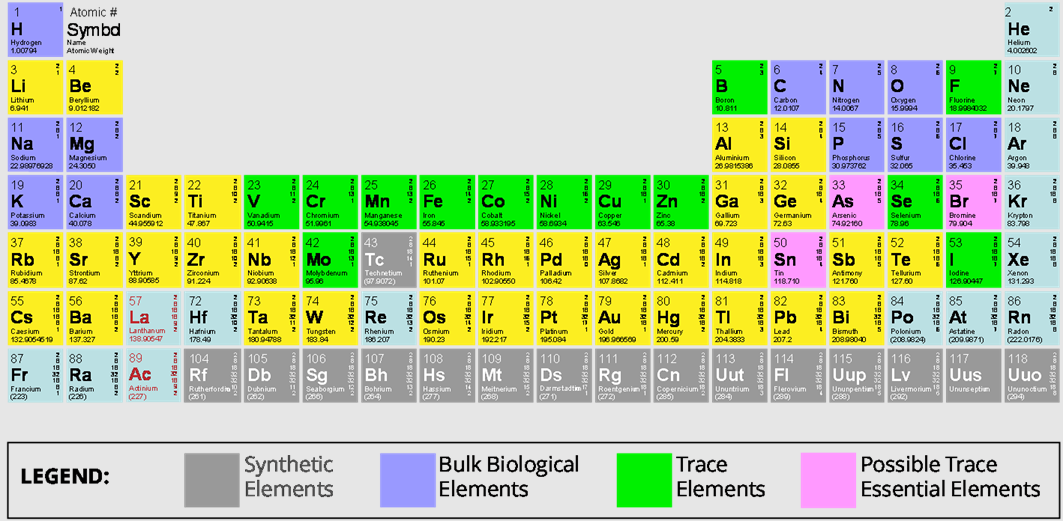
\includegraphics[width = \textwidth]{periodic-table}\]
\section{Bonds and interactions}
\label{sec:orgd554b9a}
The table below is based on the \textbf{average} values of bond strength. A reversal of the relative strengths is often found as each bond might have higher or lower strength than the average bond strength.

\begin{center}
\begin{tabular}{ |c|m{15em}|c| }
\hline
\textbf{Name} & \textbf{Basis of interaction} & \textbf{Strength} \\
\hline
Covalent bond & Sharing of electron pairs & Strongest \\
\hline
Ionic bond & Attraction of opposite charges & Strong \\
\hline
Hydrogen bond & Sharing of hydrogen atom & Relatively strong \\
\hline
Hydrophobic interaction & Forcing of hydrophobic portions of molecules together in the presence of polar substances & Weak \\
\hline
Van der Waals attraction & Weak attractions between atoms due to oppositely polarised electron clouds & Weakest \\
\hline
\end{tabular}
\end{center}

\newpage
\section{Properties of water}
\label{sec:orgb837085}
\begin{itemize}
\item Adhesion
\item Cohesion (self-adhesion of water molecules)
\item Solubilising ionic compounds
\item High specific heat capacity
\item High heat of vapourisation
\end{itemize}
\section{Common weak acids}
\label{sec:orgb544d62}
\begin{center}
\begin{tabular}{ c c c c }
\textbf{Acid} & \textbf{Conjugate Base} & $\mathbf{pK_a}$ & $\mathbf{K_a (\si{M})}$ \\
\hline
$H_3PO_4$ & $H_2PO_4^-$ & 2.14 & $7.24 \times 10^{-3}$ \\
$H_2PO_4^-$ & $HPO_4^{2-}$ & 6.86 & $1.38 \times 10^{-7}$ \\
$HPO_4^{2-}$ & $PO_4^{3-}$ & 12.4 & $3.98 \times 10^{-15}$ \\
$H_2CO_3$ & $HCO_3^-$ & 6.37 & $4.27 \times 10^{-7}$ \\
$HCO_3^-$ & $CO_3^{2-}$ & 10.25 & $5.62 \times 10^{-11}$ \\
\end{tabular}
\end{center}
\section{Diversification over time}
\label{sec:orge1852a9}

\begin{forest}
for tree={
delay = {where content = {}
{shape = coordinate, for siblings = {anchor = north}}{}},
}
[Common Ancestor (First Cell)
[Bacteria]
[Archaea]
[Eukarya (Cell with nucleus)
[Protists]
[
[Plants]
[
[Fungi]
[Animals]]]]]
\end{forest}

\newpage
\section{Classification Categories}
\label{sec:org06718a6}
The mnemonic to remember the taxonomic classifications is:


\textbf{Dear Kevin, please come over for gay sex.}


Domain, Kingdom, Phylum, Class, Order, Family, Genus, Species.


\[\text{Species}\]
\[\subset\]
\[\text{Genus}\]
\[\subset\]
\[\text{Family}\]
\[\subset\]
\[\text{Order}\]
\[\subset\]
\[\text{Class}\]
\[\subset\]
\[\text{Phylum}\]
\[\subset\]
\[\text{Kingdom}\]
\[\subset\]
\[\text{Domain}\]
\subsection{Domains}
\label{sec:org93ef94d}
The domains of life are:
\begin{itemize}
\item Archaea domain
\item Bacteria domain
\item Eukarya domain
\end{itemize}
\subsubsection{Archaea domain}
\label{sec:org8857ebb}
Contains unicellular \textbf{prokaryotes} that live in extreme environments.
\subsubsection{Bacteria domain}
\label{sec:orgfb598a2}
Contains unicellular \textbf{prokaryotes} that live in all environments. Prokaryotes \textbf{lack} a membrane-bound nucleus.
\subsubsection{Eukarya domain}
\label{sec:org9b91034}
Contains unicellular and multicellular \textbf{eukaryotes}. Eukaryotes \textbf{contain} a membrane-bound nucleus.
\subsection{Kingdoms}
\label{sec:org8872f12}
The kingdoms of life are:
\begin{itemize}
\item Plantae kingdom
\item Animalia kingdom
\item Protists kingdom
\item Fungi kingdom
\end{itemize}
\subsubsection{Plantae kingdom}
\label{sec:org1fcaf0f}
The plantae kingdom includes certain algae, mosses, ferns, conifers, and flowering plants. They are multicellular, usually with specialised tissues containing complex cells. They also photosynthesise food.
\subsubsection{Animalia kingdom}
\label{sec:org2cf351d}
The animalia kingdom include sponges, worms, insects, fishes, frogs, turtles, birds, and mammals. They are multicellular with specialised tissues containing complex cells. They ingest food.
\subsubsection{Protist kingdom}
\label{sec:org2fa5a77}
The protist kingdom include algae, protozoans, slime moulds, and water moulds. They are complex single cell organisms, and they absorb, photosynthesis or ingest food.
\subsubsection{Fungi kingdom}
\label{sec:org2c46eb0}
The fungi kingdom include moulds, mushrooms, yeasts and ringworms. They are mostly multicellular filaments with specialised, complex cells and absorb food.
\section{Virus}
\label{sec:org7aae13e}

\subsection{Similarities to living things}
\label{sec:org49974c8}
\begin{itemize}
\item It has hereditary material in the form of DNA or RNA.
\item Its offspring are carrying these material.
\end{itemize}
\subsection{Similarities to non-living things}
\label{sec:org7c97044}
\begin{itemize}
\item It does not have a cell.
\item The structure of a virus is a protein shell with a core of genetic material.
\item It can only reproduce by using the machinery of others' cells.
\end{itemize}
\subsection{Naming of viruses}
\label{sec:org6078212}
Viruses are not given genus and species names, because of its "living and non-living" nature. It follows the format, XXX virus, where XXX can be:
\begin{itemize}
\item Name of the place where the first case appeared, like Ebola (a river a Zaire), Lassa (town in Nigeria), West Nile (West of Nile River, Egypt).
\item Name of the disease or symptoms it causes, like Influenza Virus, Bird Flu Virus (Avian Influenza), SARS virus, Human Immunodeficiency Virus (HIV).
\item Others, like the name of the discoverer (Epstein-Barr virus), or the biological characteristics of the virus (vesicular stomatitis virus) etc.
\item The main name can be followed by a subtype or strain name, like Influenza A H1N1.
\end{itemize}

\newpage
\section{Levels of organisation in the human body}
\label{sec:org8af1188}
\[\text{Human body}\]
\[\downarrow\]
\[\text{Human cell}\]
\[\downarrow\]
\[\text{Chromosome}\]
\[\downarrow\]
\[\text{Gene}\]
\[\downarrow\]
\[\text{Gene expression and cell types}\]
\section{Mammalian body cavities}
\label{sec:orgc196663}

\subsection{Ventral cavities}
\label{sec:org07bc2dd}

\subsubsection{Thoracic cavity}
\label{sec:org99c2bb3}
The thoracic cavity contains the heart, lungs, and esophagus.
\subsubsection{Abdominal cavity}
\label{sec:org53180ab}
The abdominal cavity contains digestive and other organs, such as the stomach, liver, spleen, pancreas, and intestines.
\subsubsection{Pelvic cavity}
\label{sec:org5ef4547}
The pelvic cavity contains certain reproductive organs.
\subsection{Dorsal cavities}
\label{sec:orgabc0a1b}

\subsubsection{Cranial cavity}
\label{sec:orgb57d167}
The cranial cavity contains the brain.
\subsubsection{Vertebral cavity}
\label{sec:org6398c16}
The vertebral cavity contains the spinal cord.
\subsubsection{Diaphragm}
\label{sec:org466a907}
The diaphragm is a membrane-like structure of muscle, tendons and fibrous tissue that separates the thoracic cavity from the abdomen.
\section{The organ systems of humans}
\label{sec:org41d5632}

\subsection{Nervous system}
\label{sec:orgd522b90}
The nervous system functions to sense and process incoming environmental stimulus to bring about appropriate responses.
\subsection{Integumentary system}
\label{sec:orgb06c1d0}
The integumentary covers the body and consists of the skin, hair and the accessory structures of skin. It serves to protect underlying tissues against drying, physical trauma and from pathogens. It also regulates body temperature and is embedded with receptors that are responsible for sensing by the nervous system.
\subsection{Respiratory system}
\label{sec:org1ab36f4}
The respiratory system is the breathing machinery of the body.
\subsection{Endocrine system}
\label{sec:org375b59a}
The endocrine system regulates all biological processes in the body, such as the growth and function of the reproductive system and the development of the brain and nervous system, as well as the metabolism and blood sugar levels.


The endocrine system is also known as the hormone system.
\subsection{Urinary system}
\label{sec:orge70d77f}
The urinary system contains two kidneys and functions to remove metabolic waste from the body.
\subsection{Digestive system}
\label{sec:org651cd2a}
The digestive system is responsible for breaking down food substances into simpler molecules that can be absorbed.
\subsection{Reproductive system}
\label{sec:org081a943}
The reproductive system is responsible for reproduction.
\subsection{Muscular system}
\label{sec:org0eab19b}
The muscular system is responsible for bringing about motions.
\subsection{Immune system}
\label{sec:org45729ee}
The immune system consists of lymphoid organs, such as the spleen and thymus, as well as the lymphatic vessels and lymph nodes.
\subsection{Skeletal system}
\label{sec:org1cf882f}
The skeletal system forms the scaffold upon which the muscular system is layered on.
\subsection{Circulatory system}
\label{sec:org58a60db}
The circulatory system consists of heart and blood vessels and functions to transport materials such as oxygen, nutrients and wastes around the body via blood.
\end{document}
